% 
% Annual Cognitive Science Conference
% Sample LaTeX Paper -- Proceedings Format
% 

% Original : Ashwin Ram (ashwin@cc.gatech.edu)       04/01/1994
% Modified : Johanna Moore (jmoore@cs.pitt.edu)      03/17/1995
% Modified : David Noelle (noelle@ucsd.edu)          03/15/1996
% Modified : Pat Langley (langley@cs.stanford.edu)   01/26/1997
% Latex2e corrections by Ramin Charles Nakisa        01/28/1997 
% Modified : Tina Eliassi-Rad (eliassi@cs.wisc.edu)  01/31/1998
% Modified : Trisha Yannuzzi (trisha@ircs.upenn.edu) 12/28/1999 (in process)
% Modified : Mary Ellen Foster (M.E.Foster@ed.ac.uk) 12/11/2000
% Modified : Ken Forbus                              01/23/2004
% Modified : Eli M. Silk (esilk@pitt.edu)            05/24/2005
% Modified: Niels Taatgen (taatgen@cmu.edu) 10/24/2006

%% Change ``a4paper'' in the following line to ``letterpaper'' if you are
%% producing a letter-format document.

\documentclass[10pt,letterpaper]{article}

\usepackage{cogsci}
\usepackage{pslatex}
\usepackage{apacite}
\usepackage{graphicx}
\usepackage{color}


\title{Basal Ganglia-Inspired Functional Constraints Improve the Robustness of $Q$-value Estimates in Model-Free Reinforcement Learning}
 
\author{{\large \bf Patrick J. Rice (pjrice@uw.edu)} \\
  Department of Psychology, University of Washington \\
  Campus Box 351525, Seattle, WA 98195 USA
  \AND {\large \bf Andrea Stocco (stocco@uw.edu)} \\
  Department of Psychology, University of Washington \\
  Campus Box 351525, Seattle, WA 98195 USA}


\begin{document}

\maketitle

\begin{abstract}
Due to the correspondence between the striatal dopamine signal and prediction error signal utilized by model-free reinforcement learning methods, computational psychological research has found much success in modeling the basal ganglia as a biological implementation of a reinforcement learning mechanism. A large majority of these modeling efforts have focused on applying the tenets of reinforcement learning to the proposed functions of the basal ganglia, but few (if any) have attempted to apply crucial aspects of basal ganglia neurophysiology to reinforcement learning mechanisms. Here, we propose a basal ganglia-plausible model that explicitly utilizes two symmetric sets of actions (analogous to the basal ganglia's direct and indirect pathways), to simultaneously update value estimates of both available actions (i.e. chosen and not chosen) in the Probabilistic Stimulus Selection (PSS) task. We demonstrate that this proposed model architecture outperforms a standard reinforcement learning model of the PSS task by eliminating the standard model's bias towards estimation of the most valuable available actions, while granting improved resistance to noise in the internal selection process.

\textbf{Keywords:} 
Reinforcement learning; basal ganglia; dopamine; computational models
\end{abstract}


\section{Introduction}


Model-free reinforcement learning (RL) is a powerful approach for obtaining an optimal long-term action policy in the absence of transition probability and reinforcement functions. In other words, a model-free RL agent must interact with an unknown environment (i.e., sample the environment repeatedly through action) in order to construct an optimal control policy, based on the pattern of reward received by interaction with the environment. This framing of RL methods makes clear their power in modeling human and animal decision-making. Policies refined through RL mechanisms are oriented such that the agent's (i.e., human/animal) actions consider both immediate and future reward, optimized to maximize some value over time. The key idea that enables an agent to determine an optimal policy within an unknown environment is that of temporal-difference (TD) learning \cite{sutton1988learning}. 

The ideas behind TD methods have since been expanded, including a proposal by \citeA{watkins1992q} that defined a TD control algorithm now known as $Q$-learning. $Q$-learning is an off-policy method that allows the agent to choose to take non-optimal actions while still estimating an optimal value function. By updating action values based on the best action available while allowing the agent to make inferior choices, this procedure increases the rate of learning under a suboptimal action selection process. Both TD learning and Q-learning have been shown to converge to the optimal value function with probability $P = 1$ \cite{sutton1998reinforcement}.

However, in some circumstances, these model-free RL methods produce suboptimal results. As defined, these methods emphasize learning of rewarding actions -- updating the value of a state/state action (SA) pair increases the likelihood that the agent will choose the action that leads to that state/SA pair when it is next given the opportunity to do so. As a result, even though it converges to an optimal value function, an agent still does not have complete knowledge of its environment -- namely, it does not know much (if anything) about the least rewarding states/SA pairs. This is an instance of the general exploration-exploitation trade-off that many models encounter. Lacking knowledge of the least rewarding alternatives is not an issue while the agent has full access to its actions, but what if learned ``good'' (i.e. optimal) states/SA pairs are blocked from the agent? In this case, the agent cannot take the actions it usually would by following its policy and value function, and as a consequence, cannot act optimally within the ``new'' environment. In essence, the agent has no knowledge of how to navigate bad options -- how to choose the ``least bad'', when forced to.

\subsection{The Probabilistic Stimulus Selection Task}

\begin{figure*}[ht]
	\begin{center}
		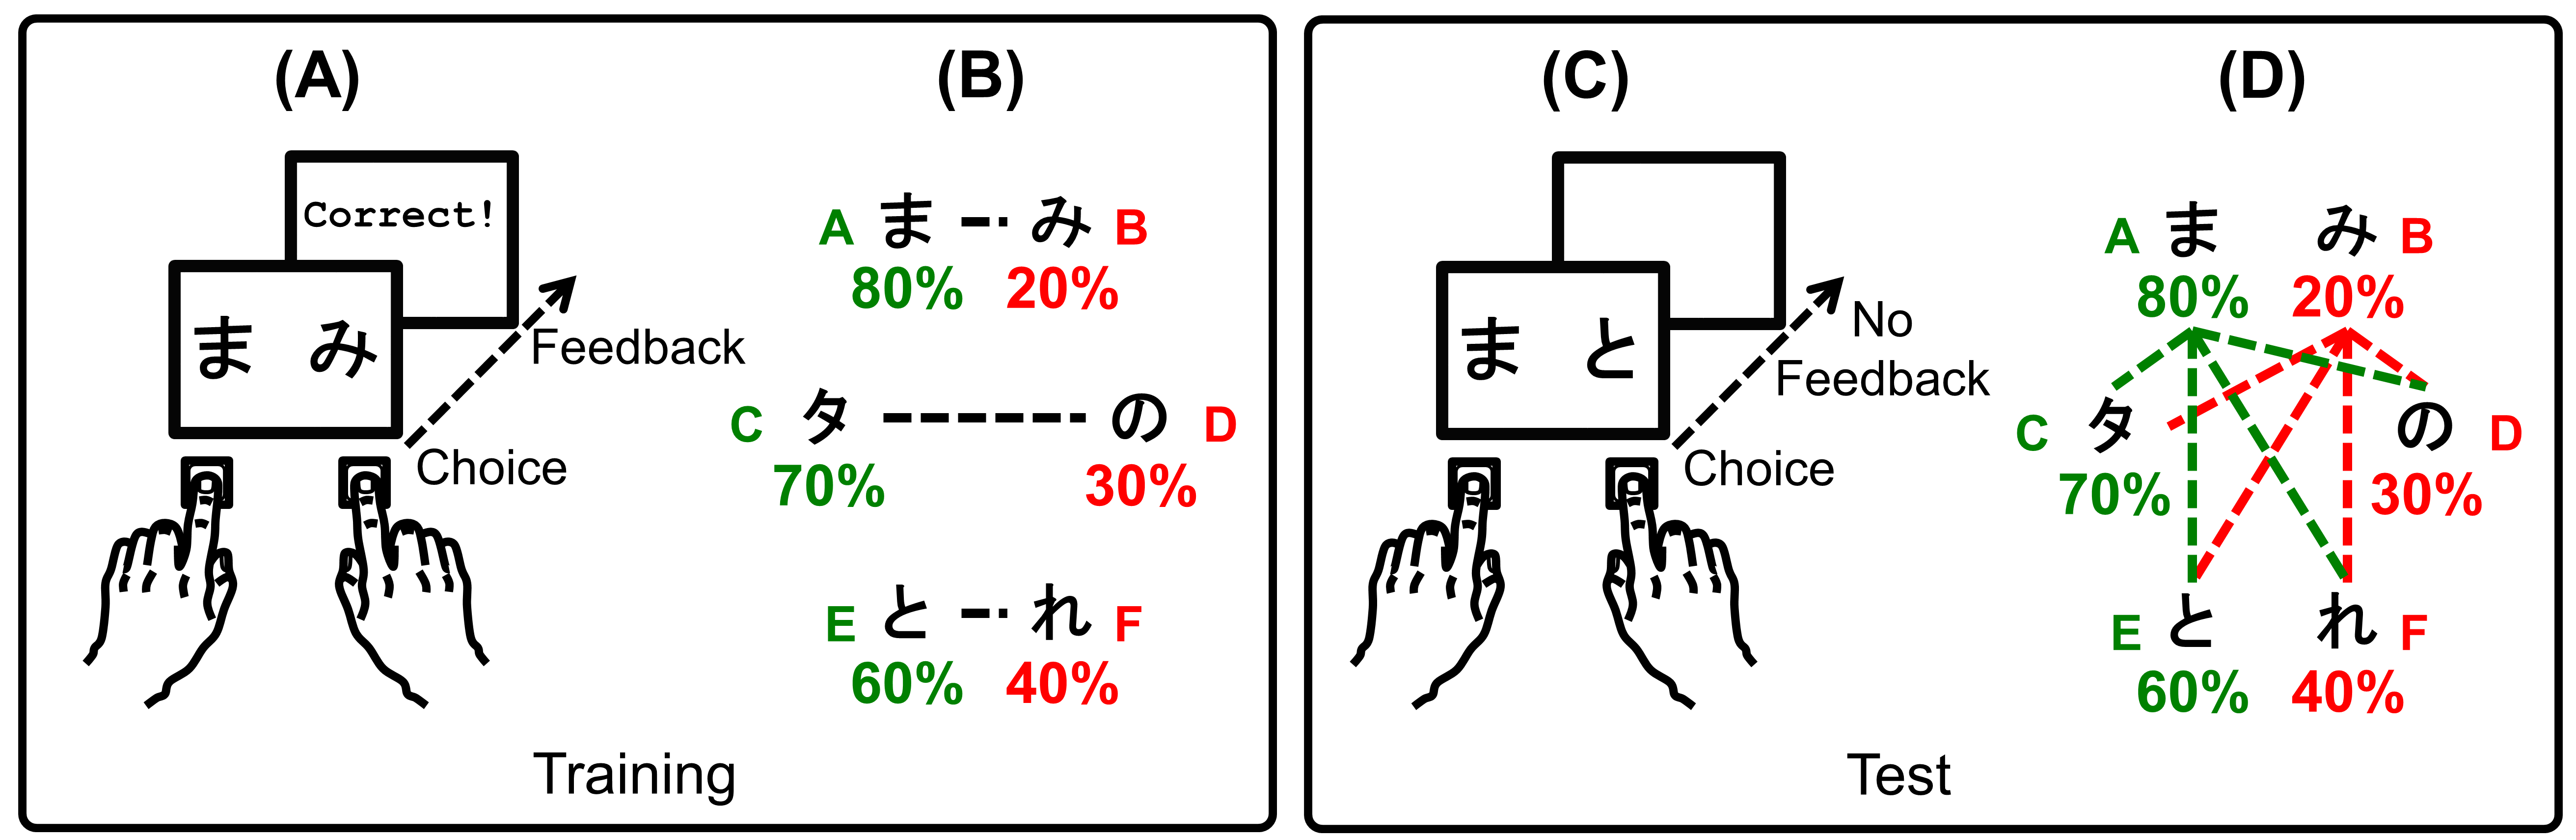
\includegraphics[width=6.5in]{pss.png}
	\end{center}
	\caption{An overview of the Probabilistic Stimulus Selection task. In the \emph{training phase}, participants learn to identify the best option within three pairs. In the ]\emph{test phase}, the six options appear in new paired combinations.}
	\label{pss}
\end{figure*}

A situation in which this circumstance arises is when modeling a well-known psychology task paradigm, the Probabilistic Stimulus Selection (PSS) task \cite{frank2004carrot}. The PSS task is a repetitive, two-alternative forced-choice task made up of two consecutive phases, a \emph{training phase} in which a participant repeatedly makes choices between fixed pairs of stimuli, and a \emph{test phase} where the participant is presented with new combinations of options (see Figure \ref{pss}).

Across both phases, there are six possible stimuli, implemented as symbols that are difficult to describe (in order to make memorization of each stimulus’ history of success more difficult). Each stimulus carries an intrinsic probability of success, ranging linearly from 20\% to 80\%. During the training phase, the stimuli are presented a fixed pairs, for a total of three sets: $(A, B)$  $(C,D)$, and $(E, F)$, with associated reward probabilities of $(80\%, 20\%)$, $(70\%, 30\%)$, and $(60\%, 40\%)$, respectively. Participants receive feedback regarding the outcome of their decision directly after making a selection, and are instructed to attempt to maximize their success by choosing what they believe to be the ``correct'' option on each trial. {\color{red} Responses that are probabilistically determined to be errors are associated with negative reward (i.e. ``feedback''), while those deemed correct are associated with positive reward, with the consequence that a component of ``good'' performance is avoiding ``bad'' (i.e. low probability of success) choices.} Once a participant's performance reached a predefined criterion (different for each pair: 65\%, 60\%, and 50\% probability of choosing the higher valued option for the sets of $(A, B)$  $(C,D)$, and $(E, F)$, respectively), the test phase begins. During the test phase, participants are shown all possible combinations of the six stimuli(fifteen total, four times each, for a total of 60 trials), and do not receive feedback upon selection. From the test phase, two different measures are calculated: the participant's \emph{Choose accuracy}, that is, the probability of choosing the highest valued alternative (A; 80\% reward probability) when it is paired with any other alternative, and the participant's \emph{Avoid accuracy}, {\color{red} that} is, the probability of not choosing the lowest valued alternative (B, 20\% reward probability) when it is paired with any other alternative (excepting A). These measures can generally be interpreted to be the participant's tendencies to pursue reward and avoid punishment, respectively.


Human participants perform close to criterion in the test phase, with an average of about 70\% accuracy in both Choose and Avoid accuracies \cite{frank2004carrot, frank2007genetic, stocco2017individual}.

\section{Model Comparisons}

\subsection{General Model Implementation}

The PSS task poses a number of important constraints for the design of RL agents. In this section, we outline these constraints, and how they were addressed in the implementation of our agents. 

The first constraint is that the set of actions available to an agent corresponds to the decision options in the task, that is, the six options $A, B \dots F$. 

The second constraint is that an agent should be able to generalize the $Q$ value of an action to an different state. This is essential to permit generalization of the $Q$-values learned during the training phase (Figure \ref{pss}A and \ref{pss}B) to the new set of pairs in the test phase (Figure \ref{pss}C and \ref{pss}D). A number of mechanisms have been proposed to generalize $Q$-values to new states. In this paper, we have taken the minimalistic approach of associating all actions to a single state $s$, but changing the set of actions available at every trial depending on the options presented. Thus, in a trial where the options $A$ and $B$ are presented, only the actions $a_A$ and $a_B$ will be selectable by the agent.

The third constraint is related to the second, and concerns the relationship between subsequent states in the PSS task. Because the PSS task consists of a sequence of \emph{independent} trials, the probability of a state $s_{t+1}$ following another state $s_{t}$ does not depend on the action taken $a_t$. Canonical RL algorithms based on temporal difference rely on the environment states to be concatenated in some way, since the update term for the $Q$-value of an action taken at state $s_t$ depends on the $Q$-value of the agent's actions at state $s_{t+1}$ For example, in the $Q$-learning algorithm, the error term depends on the \emph{best action} available at state $s_{t+1}$.

\begin{equation}
Q_{s_t,a_t} \leftarrow Q_{s_t,a_t} + \alpha [r_{t+1} + \gamma \max(Q_{s_{t+1}, a_{t+1}} - Q_{s_t,a_t})]
\end{equation}

Other algorithms, such as SARSA, similarly rely on the measuring the $Q$-value of the action taken at state $s_t$, i.e. $Q(s_{t+1}, a_{t+1})$. Since the trials are randomized, however, the contribution of the term $Q_{s_{t+1}, a}$ is going to be statistically identical, in the long term, across all states in the long-term. For convenience, in these simulations we set this term to be zero, so that the final learning equation reduces to:

\begin{equation}
Q_{s_t,a_t} \leftarrow Q_{s_t,a_t} + \alpha [r_{t+1} - Q_{s_t,a_t})]
\end{equation}

Note that, under these conditions, the $Q$-value of an action $a$ converges to the probability of reward $P(R_t)$ associated with each corresponding option.


%When the participant in the PSS task is modeled as a $Q$-learning agent %that employs a policy based on the {\color{red} softmax action selection %function:}

{\color{red} The participant's policy in the PSS task was modeled as as a Gibbs softmax action selection function:}

\begin{equation}
P(a_i) = \frac{e^{\frac{Q(a_i)}{T}}}{\sum_{j} e^{\frac{Q(a_j)}{T}}}\\.
\end{equation}

{\color{red} Under this mechanism, the probability of the agent choosing a given action increases proportionally with the action's value $Q(s,a)$, divided by a parameter $T$, defined as the \emph{temperature} of the system. Higher values of $T$ inject more noise into the action selection process, causing action selection to be less deterministic.

\subsection{Standard RL Model}

At relatively high values of $T$, where the estimated utility of actions has a smaller effect on the action selection mechanism, the RL model's Choose and Avoid accuracies are approximately equal, revealing that the model has estimated the value of choosing $A$, when presented with any option other than $B$, as approximately equal to the value of \emph{not} choosing $B$, when presented with any option other than $A$. This is desired model behavior--the model should estimate that choosing $A$ is equal to \emph{not} choosing $B$. However, as a consequence of the high level of noise in the action selection process, the model has not estimated the actual value of these two actions appropriately (relative to the value of all other options), as indicated by the low Choose and Avoid accuracies \ref{RL-agent-performance}. 

On the other hand, when the value of $T$ is low, and the action selection process is largely dependent on the estimated $Q$-values of the actions associated with the current state, some alarming results occur.} 

Specifically, the model learns the value of of the desirable options $A$, $C$, and $E$ well, reflected as a {\color{red} increasing} Choose accuracy as $T$ {\color{red} decreases} (Figure \ref{RL-agent-performance}, grey line). This is the expected behavior of the model -- {\color{red} as a deterministic action selection process based on the estimated value of actions allows exploration} to suggest relatively ``better'' options, the model quickly switches to exploiting them, learning their true values well in the process \footnote{Although here we report the results obtained using the {\color{red} softmax function}, the same results have been replicated with another common policy that balances exploration and exploitation, the $\epsilon$-greedy policy.}. 

\begin{figure}[ht]
	\begin{center}
		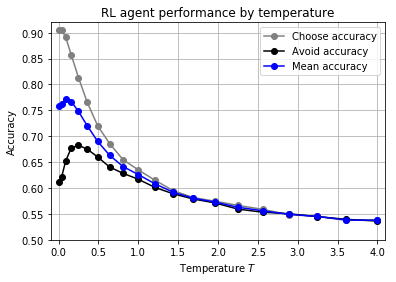
\includegraphics[width=3.5in]{rl-performance.png}
	\end{center}
	\caption{Performance of a canonical RL model in the PSS task for various levels of temperature $T$. \emph{Grey}: Choose accuracy; \emph{Black}: Avoid accuracy; \emph{Blue}: Mean accuracy.} 
	\label{RL-agent-performance}
\end{figure}



However, when the Avoid accuracy of the model is inspected, it becomes clear that the model has learned the value of some, but not all, options well. As the value of $T$ begins {\color{red} decreasing}, the Avoid accuracy of the model does begin {\color{red} increasing}, as the Choose accuracy did. However, the model's Avoid accuracy actually begins to decrease (Figure \ref{RL-agent-performance}, black line) as $T$ continues to {\color{red} decrease}. This indicates that for lower values of $T$, the model does not sufficiently explore the ``bad'' options (B, D, and F) during the training phase, and as a consequence, does not value them appropriately. For higher values of $T$, the model does explore both bad and good options approximately equally -- however, it does not value neither good nor bad options appropriately. Additionally, the maximum Avoid accuracy achieved at the point of inflection (less than 70\%) is much lower than the maximum Choose accuracy achieved by the model (which is when the value of $T$ is at a minimum; approximately 90\%), as well as the Choose accuracy at the point of inflection. 

This pattern of Choose and Avoid accuracies over the range of $T$ values tested suggests the existence of an accuracy/bias trade-off -- to become more accurate on average for a given option, the model must bias its action choices to exploiting that option (in other words, the model increases the quality of its estimates of the ``good'' options, while becoming more uncertain about the value of the ``bad'' options). This effect can be seen as tendency of RL agents to converge towards overly optimistic estimates, which has been noted in the literature \cite{hasselt2010double}. Note that this trade-off effect does not manifest in human performance. To visualize the model's trade-off issues, the model's estimate error (defined as the bias towards choosing a given option, with respect to the probability of avoiding the same option) can be plotted as a function of its mean accuracy (Figure \ref{roc}). An ideal PSS task agent would be able to obtain unbiased estimates for every level of accuracy (the vertical dashed black line). However, as made clear by Figure \ref{roc}, the model's estimate error increases as mean accuracy increases--the model becomes more uncertain about it’s ``bad'' options in order to do well when presented with ``good'' options.

\begin{figure}[ht]
	\begin{center}
		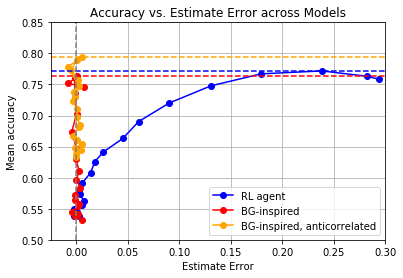
\includegraphics[width=3.5in]{roc-agents.png}
	\end{center}
	\caption{Mean accuracy vs. $Q$-value estimate errors for the three models examined in this paper. Solid lines indicate the accuracy-error trade-off curves; dotted lines indicate the maximum mean accuracy for each model. \emph{Blue}: Standard RL model; \emph{Red}: BG-inspired model; \emph{Yellow}: Anti-correlated BG-inspired model. } 
	\label{roc}
\end{figure}

%% THIS SHOULD PROBABLY BE REMOVED
Another way in which this apparent accuracy/bias trade-off can be demonstrated is by defining the model so that it learns the value of NOT choosing actions, rather than the value of choosing actions. In other words, the model chooses to ``not choose'' a given option, learning the value of such in the process. In this case, as the value of $T$ increases, Avoid accuracy decreases while Choose accuracy exhibits the inflection behavior seen in Avoid accuracy under the original model. Now, the model has learned how to navigate amongst ``bad'' options--it knows the value of not choosing a given option, and so it ``doesn't choose'' the ``bad'' options more often as $T$  decreases. However, it does not learn about the value of ``good'' options during the learning process.

\subsection{Basal Ganglia-Inspired RL Model}

Reinforcement learning is known to be a reliable method of modeling the function of the basal ganglia (BG) system, a network of subcortical nuclei including the striatum, globus pallidus, substantia nigra, and subthalamic nucleus \cite{alexander1990function}.

\begin{figure}[ht]
	\begin{center}
		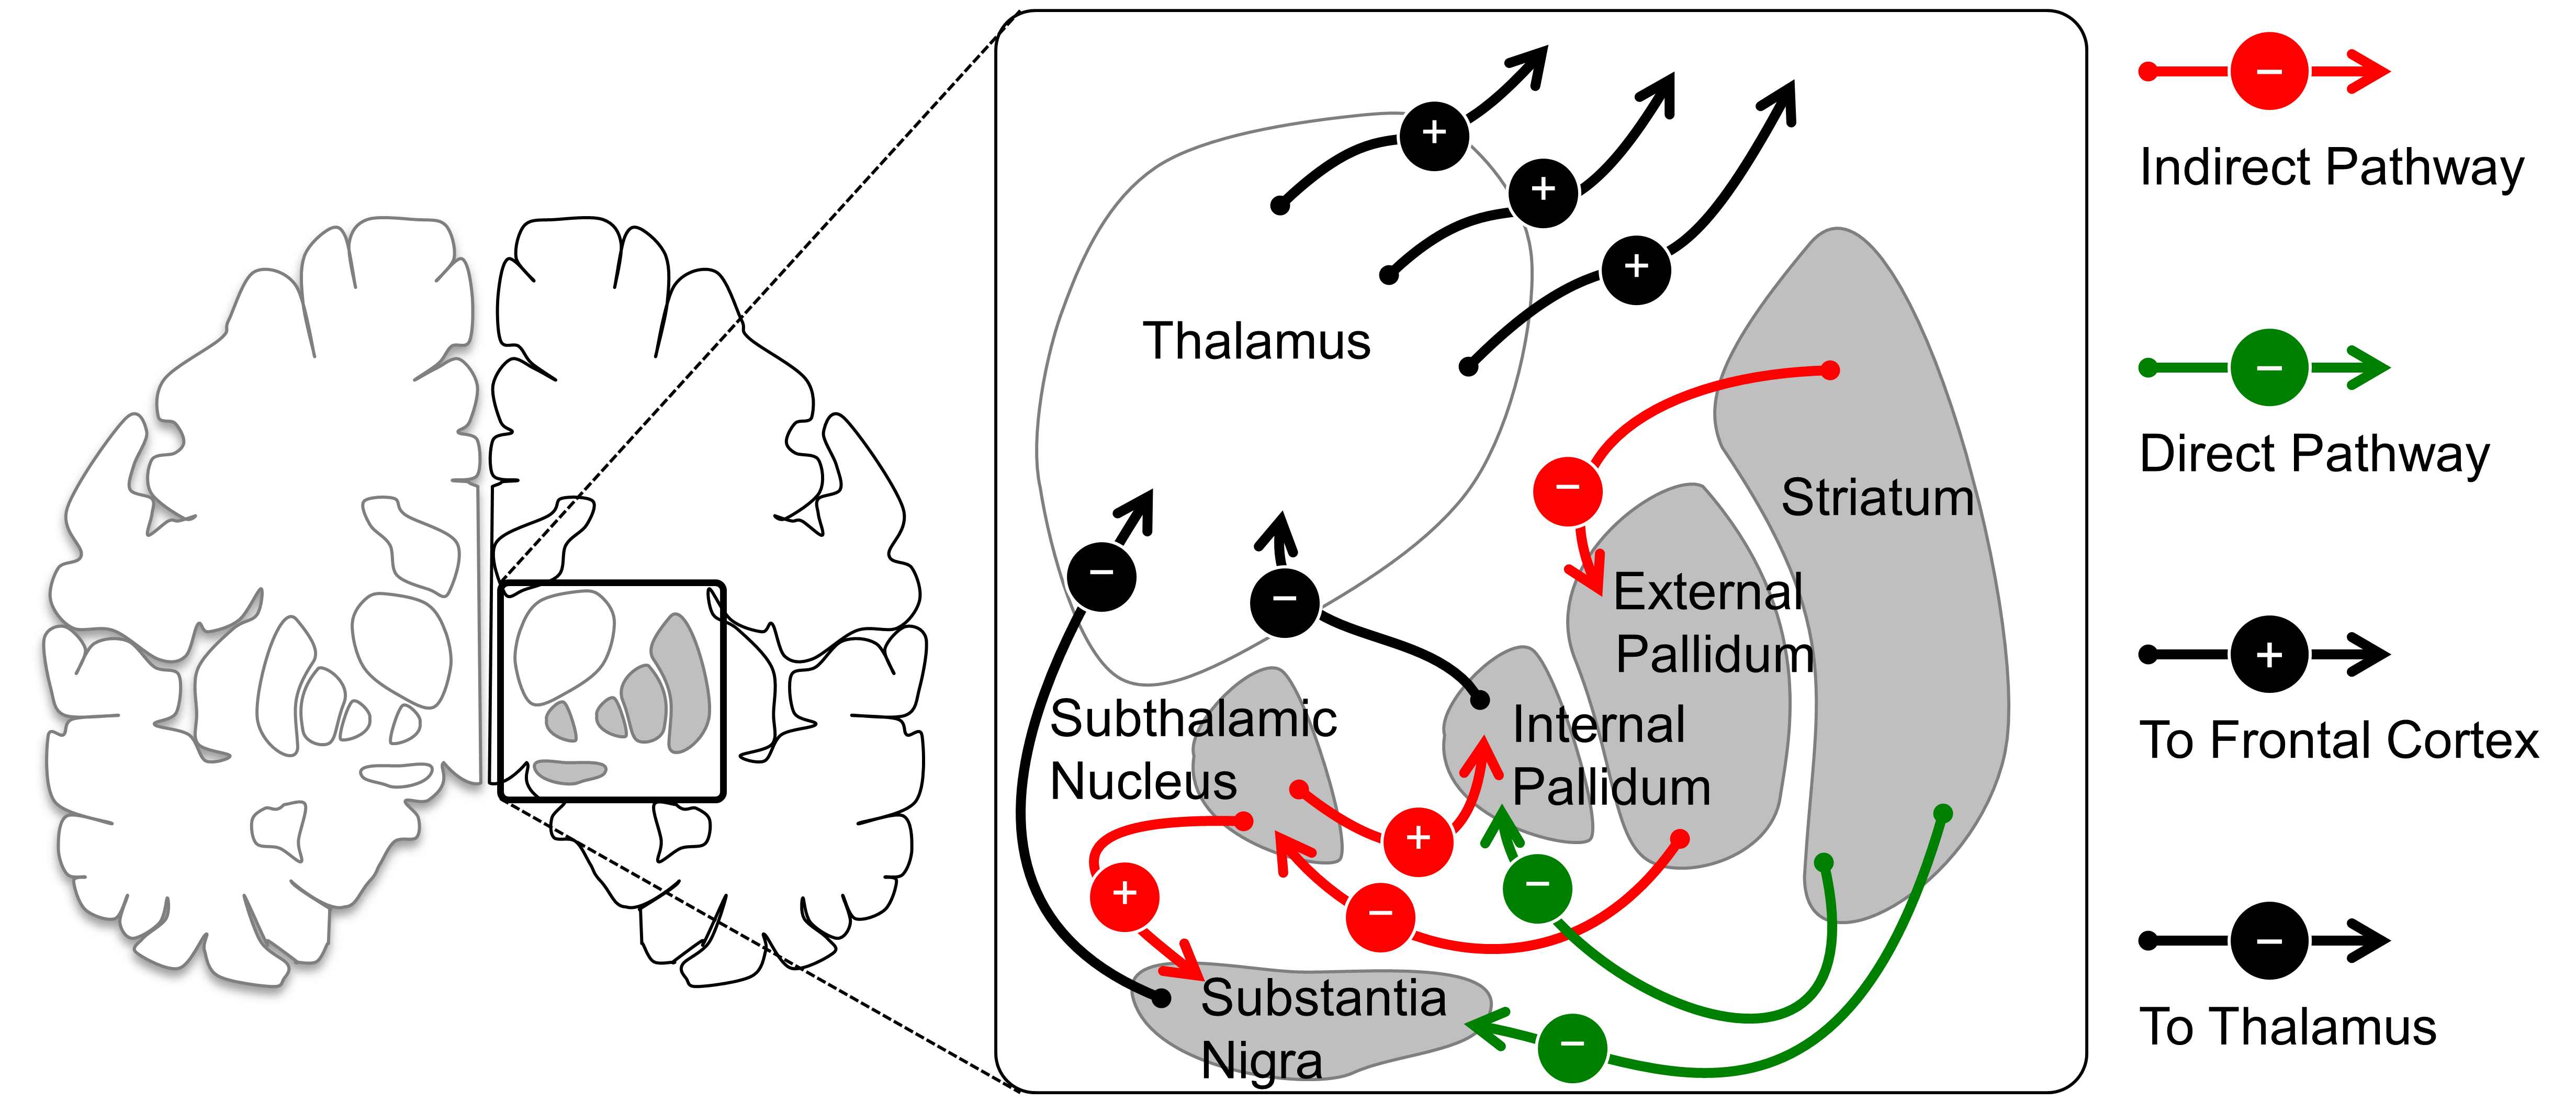
\includegraphics[width=3.5in]{basal-ganglia.png}
	\end{center}
	\caption{Overview of functional anatomy of the basal ganglia. The main basal ganglia nuclei are in grey; the arrows indicate the major projections between nuclei. The indirect pathway is shown in red, while the direct pathway is shown in green.} 
	\label{bg}
\end{figure}

The striatum receives input from cortical structures, and subsequently propagates the signal to later nuclei of the BG through two distinct pathways, termed the ``direct'' and ``indirect'' pathways \cite{smith1998microcircuitry}. Of particular interest to neurological/psychological research is the fact that the striatum also receives strong dopaminergic (dopamine; DA) input from the substantia nigra $pars compacta$ (SNc). Dopaminergic signaling originating from the SNc has long been thought to reflect a neural ``reward'' signal associated with internally-generated action and external stimuli that the organism has learned is (or expects to be) rewarding in some manner, and corresponds closely with the prediction error signal utilized in RL methods \cite{schultz2000multuple, schultz1997neural}. Additionally, dopaminergic input is a defining characteristic of the ``direct'' and ``indirect'' pathways mentioned above -- striatal neurons that express D1 receptors (for which DA is an excitatory ligand) form the origin of the direct pathway, while those that express D2 receptors (for which DA is an inhibitory ligand) form the origin of the indirect pathway.

For the PSS task, although the standard RL model does fairly well overall (approximately 77\%), its performance does not match that of human participants, especially when considering Avoid accuracy. As the model's results demonstrate, it learns well about one set of options (either the ``good'' options or the ``bad'' options, depending on if it is learning what to choose or what to not choose, respectively), but it does not do well at valuing all options appropriately at all values of $T$. Ideally, the model could instead learn the values of choosing an option and not choosing the alternative simultaneously, allowing it to train once in order to appropriately value all possible options. Superficially, there seems to be an obvious compatibility between the necessity for a RL model to simultaneously estimate the value both the ``chosen" and ``not chosen'' alternatives within a PSS trial, and dopamine's opposing influence on the direct and indirect pathways. Would a model-free RL agent with two ``action pathways'' perform any better than the standard RL model described above?

In order to implement the two-pathway concept, the $Q$-learning agent described above was modified to include an opposite set of ``don't'' actions ($\neg A, \neg B, \dots, \neg F$), which, when chosen by the agent, result in the selection of the other option that they are paired with. Thus, this agent contains a double set of actions and a stores a double set of $Q$-values; in this, it is reminiscent of double $Q$-learning \cite{hasselt2010double,van2016deep}, an algorithm devised to address the overly-optimistic estimates of the original $Q$-learning algorithm \cite{watkins1992q}.

The original set of actions ($A, B, \dots, F$) can be conceptualized as the set of actions available to be suggested by the direct pathway (restricted by actions possible within the current state), while the ``antiset'' can be conceptualized as the set of actions available to be suggested by the indirect pathway (also restricted by the state). So, if the current trial allows for actions $A$ and $B$, and the agent selects the indirect pathway's action $\neg A$, the result is the selection of option $B$. However, if the current trial allows for actions $A$ and $C$, and the agent selects $\neg A$, the result is the selection of option $C$.

\begin{figure}[ht]
	\begin{center}
		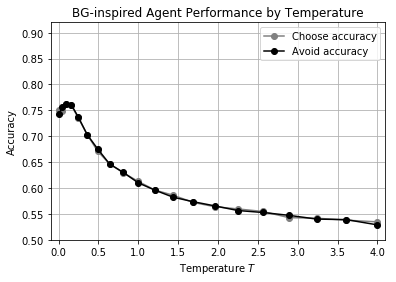
\includegraphics[width=3.5in]{bg-agent-performance.png}
	\end{center}
	\caption{Performance of the BG-inspired reinforcement learning agent in the PSS task for various levels of temperature $T$. Note that there is no difference in the Choose \emph{Grey} and Avoid \emph{Black} accuracies.}
	\label{bg-agents}
\end{figure}

Figure \ref{bg-agents} shows that the simple addition of an ``indirect pathway'' to the RL model results in a marked absence of the bias observed in the standard RL model--as the value of $T$ decreases, both choose and avoid accuracies increase commensurately. As such, the model no longer needs to ``trade-off'' increasing the accuracy for one class of action by becoming less confident in the valuations of the other class of action. Instead, for every choice made, it simultaneously learns both the value of the option chosen, and the value of not choosing the alternative. However, note that the maximum Choose and Avoid accuracies of the BG-plausible model do not quite achieve the same level of accuracy as the standard RL models--the uncertainty that the standard model had been attributing to the option not chosen has now been distributed across both available options.  Figure \ref{roc} demonstrates that overall, the BG-plausible model (red line) achieves essentially the same level of global mean accuracy as the standard RL model (blue line), but \emph{without} the cost of increasing estimate error.  


\subsection{Making the Model More Plausible}

As described, this implementation of ``direct'' and ``indirect'' pathways in the RL model does well at capturing the competition between the direct and indirect pathways of the BG, and alleviates the problem of increasing estimate error with increasing accuracy. However, the BG-plausible model still performs similarly to the standard RL model in terms of global mean accuracy, indicating that although the BG-plausible model has improved ability to estimate the value of all options in the environment, this does not translate to improved fitness within the environment. However, just as the standard models were missing a crucial aspect of BG physiology (the presence of dual pathways), the BG-plausible model is missing a crucial feature of these dual pathways -- the fact that DA signaling has opposite effects on the direct (excitation, mediated through D1 receptors) and indirect (inhibition, mediated through D2 receptors) pathways. 

To capture this aspect of BG neurodynamics, the BG-plausible RL model was modified so that the learning algorithm results in \emph{opposite} changes for the actions to the two pathways (an anti-correlated BG-plausible model). Specifically, if action $A$ was selected and resulted in an update  of it $Q$-value of size $\delta$, then the $Q$-value of the corresponding anti-action $\neg A$ would be updated by the quantity $-\delta$. As in the biological BG, this mechanism forces the values of one set of actions to be anti-correlated to the values of the other set.

Figure \ref{bg-anti-agent} shows the results of simulations ran with this model. At minimum values of $T$, the maximum mean Choose and Avoid accuracies increase slightly (when compared to the original BG-plausible model). Figure \ref{roc} shows that, similar to the original BG-plausible model (red line), the mean accuracy of the anti-correlated BG-plausible model (yellow line) increases without a subsequent increase in estimate error. Additionally, the small increase in Choose and Avoid accuracies at minimum values of T translate into significantly better overall performance for the anti-correlated BG-plausible model. 

\begin{figure}[ht]
	\begin{center}
		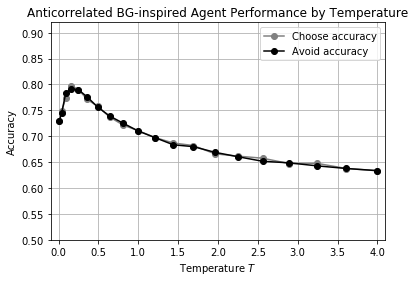
\includegraphics[width=3.5in]{bg-anti-agent-performance.png}
	\end{center}
	\caption{Performance of the anti-correlated, BG-inspired RL-learning model in the PSS task for various levels of temperature $T$.}
	\label{bg-anti-agent}
\end{figure}

However, what is most striking about the anti-correlated BG-plausible model is that at relatively large values of $T$ (where the action selection process is noisy), the model performs much better than either the original BG-plausible model, or the standard RL models. This is an indication that the presence of the anti-correlated pathways in the second BG-plausible model bestow a greater resistance to internal noise than the original BG-plausible model and standard RL models possess. Figure \ref{resistance-to-noise} more clearly demonstrates this effect: across the range of tested values of $T$, the mean accuracies of the original BG-plausible model are almost identical to the standard RL model. However, across the same range of $T$ values, the anti-correlated BG-plausible model performs much better in almost every circumstance.

\begin{figure}[ht]
	\begin{center}
		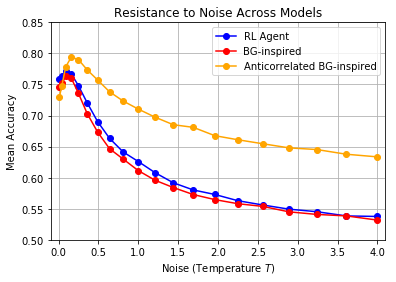
\includegraphics[width=3.5in]{resistance-to-noise.png}
	\end{center}
	\caption{A direct comparison of the mean accuracy of three RL models tested in this paper. \emph{Blue}: Standard RL model; \emph{Red}: BG-inspired model; \emph{Yellow}: Anti-correlated BG-inspired model.} 
	\label{resistance-to-noise}
\end{figure}

The model does not perform as well as the standard ``original'' BG-inspired model only when the value of $T$ is very close to zero, indicating almost no noise in the action selection process (an unrealistic assumption for biological systems). A similar analysis can be performed for the model's estimate error, as seen in Figure \ref{roc}. This again shows that for every tested value of $T$, there is little or no difference between either BG-plausible model--the presence of the two pathways allows each model to accurately estimate the value of both the most rewarding ($A$, $C$, and $E$) and least rewarding ($B$, $D$, and $F$) options. However, the standard RL model shows significant estimation biases as the lowest levels of noise, when the model's performance is at a maximum.

\section{Conclusions}

In conclusion, the improved performance of the BG-plausible RL models implies that psychological researchers looking to model the functions of the basal ganglia could do well by taking inspiration from the characteristics of the phenomena they model, even when the modeling effort is largely theoretical. The addition of opposed action sets, representative of the well-known direct and indirect pathways within the basal ganglia, allowed the original BG-plausible model to properly estimate the value of both the ``good'' (relatively high probability of reward) and ``bad'' (relatively low probability of reward) options available in the PSS task, eliminating the bias towards ``good'' options displayed by the standard RL model. Furthermore, by forcing the updates of the two action sets to be anti-correlated (thereby mimicking the opposed excitatory/inhibitory effect of dopamine on the direct and indirect pathways), the model displayed a marked resistance to greater levels of noise within the selection mechanism.    

\section{Acknowledgments}

This research was suported by a grant from the Office of Naval Research (ONRBAA13-003) entitled ‘‘Training the Mind and Brain: Investigating Individual Differences in the Ability to Learn and Benefit Cognitively from Language Training'' and by a start-up grant from the University of Washington to Andrea Stocco. Simulations and code for this study can be found at the Cognition and Cortical Dynamics Laboratory's {\color{red} GitHub} repository: https://github.com/UWCCDL/BGRL.

\bibliographystyle{apacite}

\setlength{\bibleftmargin}{.125in}
\setlength{\bibindent}{-\bibleftmargin}

\bibliography{rice_stocco_iccm2017}


\end{document}
